\documentclass{jarticle}

\usepackage[dvipdfmx]{graphicx}
\usepackage{url}
\usepackage{listings,jlisting}
\usepackage{ascmac}
\usepackage{amsmath,amssymb}

%ここからソースコードの表示に関する設定
\lstset{
    basicstyle={\ttfamily},
    identifierstyle={\small},
    commentstyle={\smallitshape},
    keywordstyle={\small\bfseries},
    ndkeywordstyle={\small},
    stringstyle={\small\ttfamily},
    frame={tb},
    breaklines=true,
    columns=[l]{fullflexible},
    numbers=left,
    xrightmargin=0zw,
    xleftmargin=3zw,
    numberstyle={\scriptsize},
    stepnumber=1,
    numbersep=1zw,
    lineskip=-0.5ex
}
%ここまでソースコードの表示に関する設定 

\title{知能プログラミング演習II 課題3}
\author{グループ07\\
    29114007 池口 弘尚\\
    29114031 大原 拓人\\
    29114048 北原 太一\\
    29114086 飛世 裕貴\\
    29114095 野竹 浩二朗\\
%  {\small (グループレポートの場合は、グループ名および全員の学生番号と氏名が必要)}
}
\date{2019年11月5日}

\begin{document}
\maketitle

\paragraph{提出物} このレポート グループプログラム"group07.zip"
\paragraph{グループ} グループ07

\section{課題の説明}
\begin{description}
    \item[必須課題3-1] セマンティックネットのプログラムを参考に,
    グループメンバー全員(およびその周辺人物)についてのセマンティックネットを構築せよ.
    個人レポートには自分のみ(とその周辺)に関するセマンティックネットを示し,
    グループレポートには全員(とその周辺)に関するセマンティックネットを示せ.
    \item[必須課題3-2] フレームのプログラムを参考に,自分達の興味分野に関する
    知識をフレームで表現せよ.その分野の知識を表す上で必須となるスロットが
    何かを考え,クラスフレームを設計すること.
    個人レポートには自分が作ったインスタンスフレームのみ(クラスフレームの
    設計担当者はクラスフレームも)を示し,グループレポートにはクラスフレーム
    および全員分のインスタンスフレームを示せ.
    \\ 注: クラスフレームの設計についてはグループ内で共通にし,
    「メンバー毎にスロット定義がバラバラ」等ということがないよう気をつけること.
    \item[必須課題3-3] 課題3-1または3-2で作った知識表現を用いた質問応答システムを作成せよ.
    \\ なお,ユーザの質問は英語や日本語のような自然言語が望ましいが,難しければ課題2で扱ったような変数を含むパターン (クエリー) でも構わない. 
\end{description}


\section{課題3-1}
\begin{screen}
    セマンティックネットのプログラムを参考に,
    グループメンバー全員(およびその周辺人物)についてのセマンティックネットを構築せよ.
    個人レポートには自分のみ(とその周辺)に関するセマンティックネットを示し,
    グループレポートには全員(とその周辺)に関するセマンティックネットを示せ.
\end{screen}
\subsection{手法}
    グループのメンバーでそれぞれ自身に関係するセマンティックネットを構築した。
\subsection{実装-29114007 池口弘尚}
主に自分とその所有物や関係に関するセマンティックネットを構築した。
それは以下のようになった。

\begin{figure}[!hbt]
  \centering
  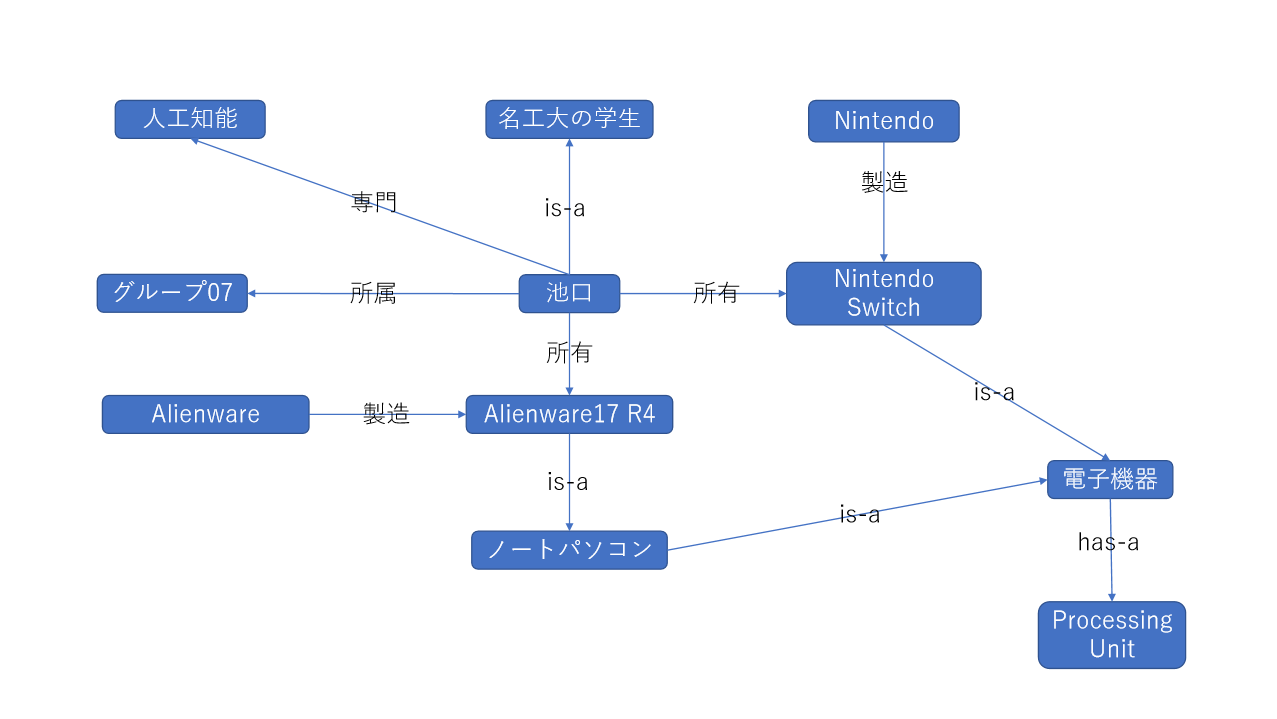
\includegraphics[bb=0 0 1277 719,width=1.2\linewidth]{007/semNet.png}
  \caption{セマンティックネット}
  \label{fig:semNet}
\end{figure}
\subsection{考察-29114007 池口弘尚}
グループでまとめる手間を省くため、できるだけ小さな要素でまとめられるようにした。
グループ07という要素はメンバー全体で共通すると思われるので、入れることにした。
また、電子機器でSuperクラスの要素も継承しているか確かめることができるようにした。
\subsection{実装-29114031大原拓人}
    自分に関するセマンティックネットは以下のようになった。
\begin{center}
    \includegraphics[scale=0.3]{031/kadai3SN.pdf}
\end{center}
\subsection{考察-29114031大原拓人}
    出身地と、所有する携帯の種類は上位クラスが共通しそうな
    項目として加えた。ほかの項目は自分の趣向に合わせて作ったので、
    グループのメンバーと共通するものはほとんどなかった。
\subsection{実装-29114086 飛世裕貴}
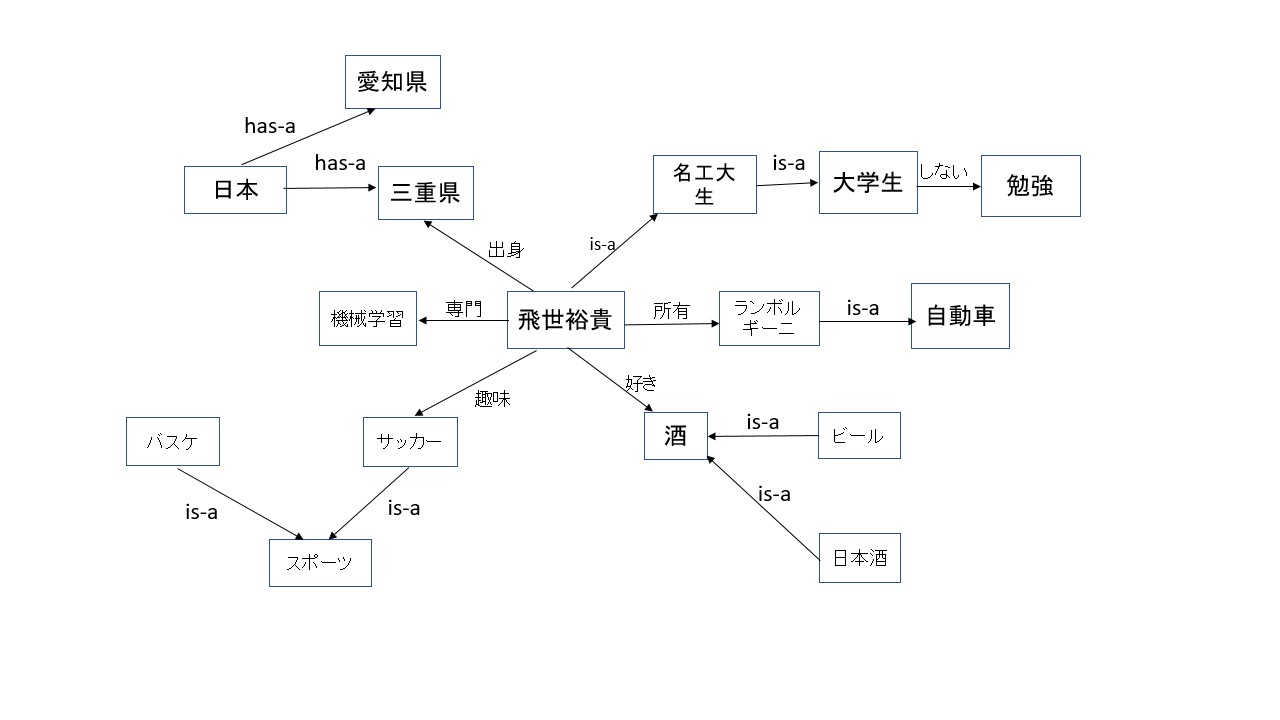
\includegraphics[width=150mm,height=80mm]{086/Slide2.jpg}
上に示したセマンティックネットをMakeSemanticNet.javaにおいて生成する.セマンティックネットの生成はExample.javaを元に実装した.

\subsection{実行例-29114086 飛世裕貴}
MakeSemanticNet.javaによってセマンティックネットを生成した.その結果を以下に示す.

\begin{screen}
\begin{verbatim}
飛世裕貴  =is-a=>  名工大生
飛世裕貴  =所有=>  ランボルギーニ
飛世裕貴  =好き=>  酒
飛世裕貴  =趣味=>  サッカー
飛世裕貴  =専門=>  機械学習
飛世裕貴  =出身=>  三重県
名工大生  =is-a=>  大学生
( 飛世裕貴  =is-a=>  大学生 )
大学生  =しない=>  勉強
( 名工大生  =しない=>  勉強 )
( 飛世裕貴  =しない=>  勉強 )
ランボルギーニ  =is-a=>  自動車
ビール  =is-a=>  酒
日本酒  =is-a=>  酒
サッカー  =is-a=>  スポーツ
バスケ  =is-a=>  スポーツ
日本  =has-a=>  三重県
日本  =has-a=>  愛知県
\end{verbatim}
\end{screen}

このように図に示したものと同様のセマンティックネットが生成されたことを確認した.

\subsection{考察-29114086 飛世裕貴}
今回生成したセマンティックネットはデータ同士の関係を記述する上で、有用なものであると考える.プログラミング言語において、データ同士の構造的関連を記述する機能は存在するが、セマンティックネットにおいては構造的な繋がりのみでなく意味的な繋がりについても記述することができる.例えば、Javaにおいてクラスを用いる事でデータの包含関係を記述する事ができるがそのデータ同士が意味的にどのような繋がりがあるか理解するためには人間がコードを見て理解する以外にないだろう.しかし、セマンティックネットにおいてはデータ同士のつながりを表すリンクに構造的関係だけでなく意味的関係を持たせている為、人間にも理解しやすく、また人間が用いる自然言語の意味推論や知識構造を表現する上で効果的なデータ構造と言える.

\subsection{実装-29114095 野竹浩二朗}
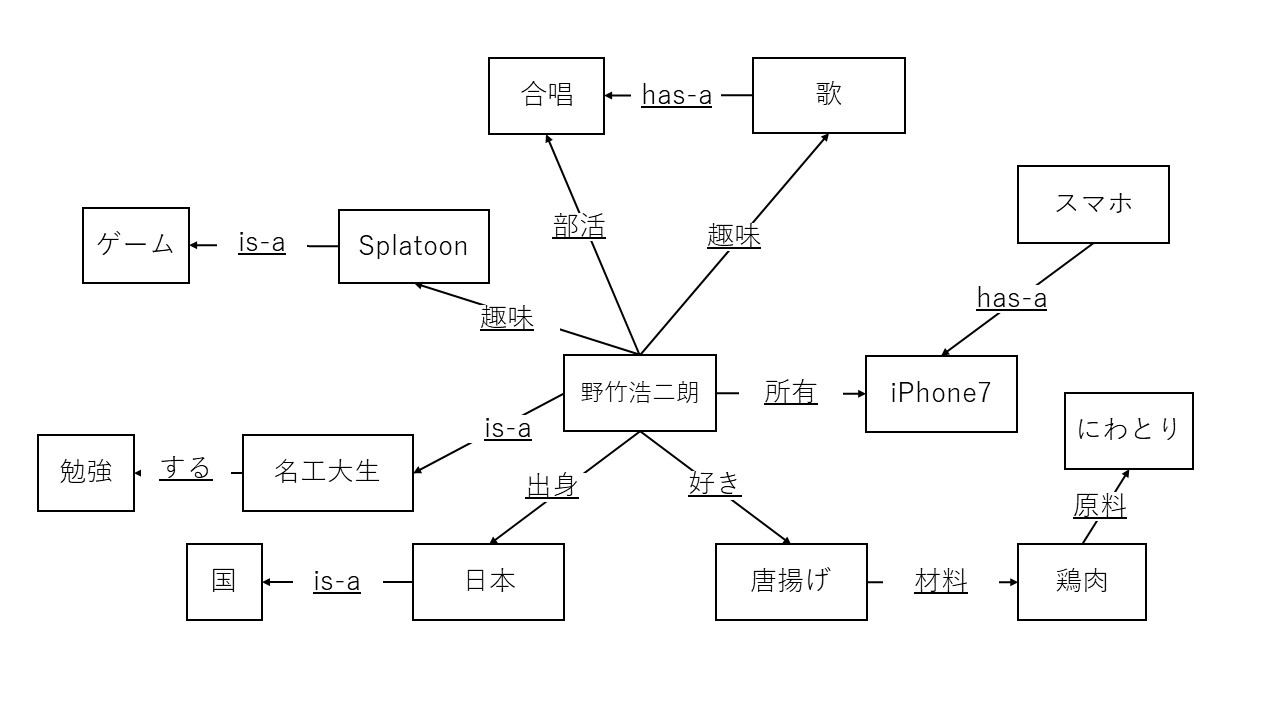
\includegraphics[width=150mm,height=80mm]{095/Semantic-Kojiro.jpg}

上に示した画像のセマンティックネットをExample.javaを参考に生成する。

\subsection{実行例-29114095 野竹浩二朗}
MakeSemanticNet.javaによってセマンティックネットを生成した.その結果を以下に示す.\\
(グループ用の出力と一致するためここでは割愛させていただく)

\subsection{実行例-グループ}
グループ用にMakeSemanticNet.javaを書き換えて実行した。
\begin{lstlisting}
    Enter Search Pattern:鶏肉,原料,?x
    *** Links ***
    飛世裕貴  =だ=>  名工大生
    飛世裕貴  =所有=>  ランボルギーニ
    飛世裕貴  =好き=>  酒
    飛世裕貴  =趣味=>  サッカー
    飛世裕貴  =専門=>  機械学習
    飛世裕貴  =出身=>  三重県
    名工大生  =だ=>  大学生
    大学生  =しない=>  勉強
    ランボルギーニ  =だ=>  自動車
    ビール  =だ=>  酒
    日本酒  =だ=>  酒
    サッカー  =だ=>  スポーツ
    バスケ  =だ=>  スポーツ
    日本  =持つ=>  三重県
    日本  =持つ=>  愛知県
    ...
    (一致しとことは確認したので省略)
    ...
    唐揚げ  =材料=>  鶏肉
    鶏肉  =原料=>  鶏
    日本  =だ=>  国
    *** Nodes ***
    飛世裕貴
    名工大生
    ランボルギーニ
    酒
    ...
    (一致しとことは確認したので省略)
    ...
    唐揚げ
    鶏肉
    鶏
    国
    *** Query ***
    鶏肉  =原料=>  ?x
    [{?x=鶏}]
\end{lstlisting}

\section{課題3-2}
\begin{screen}
    フレームのプログラムを参考に,自分達の興味分野に関する
    知識をフレームで表現せよ.その分野の知識を表す上で必須となるスロットが
    何かを考え,クラスフレームを設計すること.
    個人レポートには自分が作ったインスタンスフレームのみ(クラスフレームの
    設計担当者はクラスフレームも)を示し,グループレポートにはクラスフレーム
    および全員分のインスタンスフレームを示せ.
    \\ 注: クラスフレームの設計についてはグループ内で共通にし,
    「メンバー毎にスロット定義がバラバラ」等ということがないよう気をつけること.
\end{screen}
\subsection{手法}
グループで共通させる項目を決めた上で、いくつかの
ゲームに出現するキャラクターについてクラスフレームを作成した。
\subsection{実装-29114007 池口弘尚}
主にスマブラに関係するキャラクターを調べて、それをフレームで表した。
クラスフレームの設計が人によって異なることが無いようにメンバーの飛瀬君が作ったクラスフレームをもとに作成した。

それは以下のようになった。

\begin{figure}[!hbt]
  \centering
  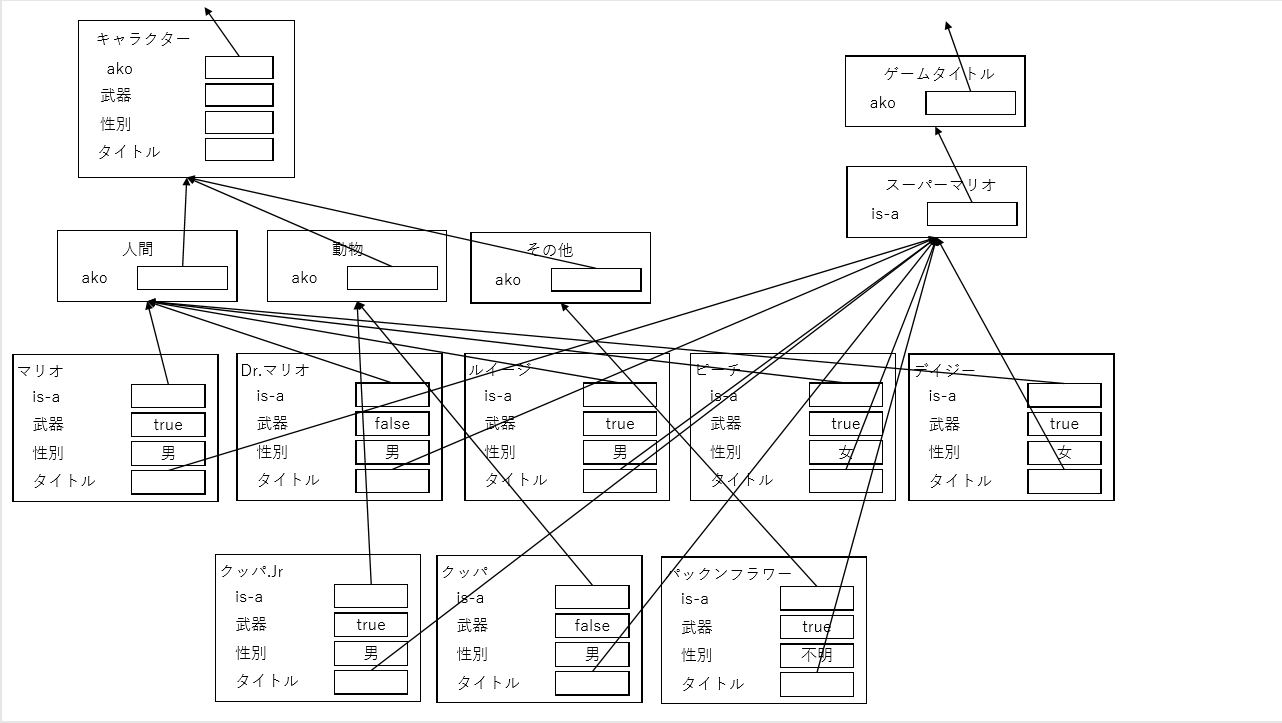
\includegraphics[bb=0 0 1282 723,width=1.2\linewidth]{007/Frame.png}
  \caption{フレーム}
  \label{fig:Frame}
\end{figure}

\subsection{考察-29114007 池口弘尚}
それぞれのキャラを探索するには特徴数が少なくなってしまった。
マリオとルイージ、ピーチとデイジーに関しては、持っているものが同じであるため、探索するのは難しいと思われる。
そのため、より多くの特徴をつける必要があると考えられる。

\subsection{実装-29114031大原拓人}
    グループで共通させる項目を決めた上で、私はポケモンのキャラクターに
    関する以下のようなクラスフレームを作成した。
    \begin{center}
        \includegraphics[scale=0.3]{031/kadai3pokemon.pdf}
    \end{center}
\subsection{考察-29114031大原拓人}
    話題をゲームのキャラクターにすることで、タイトル、性別、武器の有無、
    登場するゲームタイトルという、キャラクターが思いつけばすぐに
    スロットの値がわかる項目を設定することができた。
\subsection{実装-29114086 飛世裕貴}
ここでは任天堂の『大乱闘スマッシュブラザーズ』というゲームのキャラクターに関するクラスフレームとインスタンスフレームを構築した.構築したフレームは下図のようなものである.


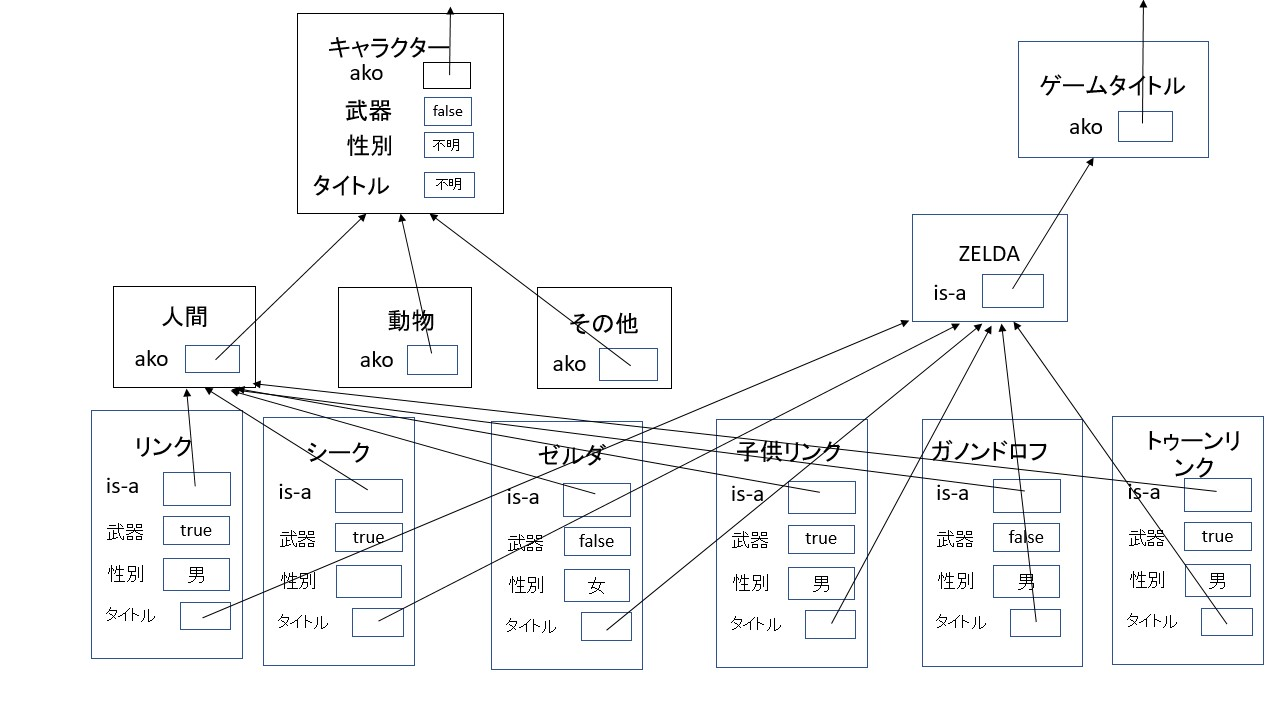
\includegraphics[width=150mm,height=80mm]{086/Slide1.jpg}

この図において「キャラクター」「人間」「動物」「その他」「ゲームタイトル」フレームをクラスフレーム、それ以外をインスタンスフレームとして構築している。\\
上に示したフレームをMakeFrame.javaにおいて生成する.フレームの生成はExample.javaを元に実装した.なおフレームの構築
において、キャラクターのスロットにゲームタイトルのインスタンスフレームを格納する必要があったため、生成したフレームを格納しているHashMapからフレームを取り出すgetFrameメソッドをAIFrameSystem.javaに、フレームの名前を取得するgetmNameメソッドをAIFrame.javaに実装した。
\subsection{実行例-29114086 飛世裕貴}
MakeFrame.javaによってフレームを生成した.ここではreadSlotValueメソッドを用いて、生成したフレームにおいて各スロットの値が正しく格納されているかを確認した.その結果の一部を以下に示す.
\\

\begin{screen}
\begin{verbatim}
Frame:リンク
武器:true
性別:男
タイトル:ZELDA
\end{verbatim}
\end{screen}

このように生成したフレームのスロットに正しい値が格納されていることがわかる.また、ここでは『リンク』フレームに関する実行結果のみを示しているが、他のフレームに関しても同様の処理をした結果、図に示したものと同様のフレームが生成されたことを確認した.

\subsection{考察-29114086 飛世裕貴}
今回生成したフレームはJavaにおけるクラスの論理構造と酷似する点が多い.
例えば、フレームにおけるスロットはクラスにおけるクラス・インスタンス変数に
相当し、フレームのクラス・インスタンスフレームの関係はそのままクラス・
インスタンスや継承に相当する.しかし、構築されるネットワークが複雑になれ
ばなるほどクラスのみを用いて実装することは困難になり、フレームやスロット
の追加はフレームの方が容易になることが予想できる.今回のように小規模のネットワーク
ではこの効力があまり実感できなかったが、自然言語の意味推論や現実世界の
知識構造のように巨大なネットワークを構築する際には効力を発揮すると考える。
\subsection{実装-29114095 野竹浩二朗}
ここでは任天堂の『大乱闘スマッシュブラザーズ』というゲームのキャラクターに
関するクラスフレームとインスタンスフレームを構築した.構築したフレームは下図のようなものである.


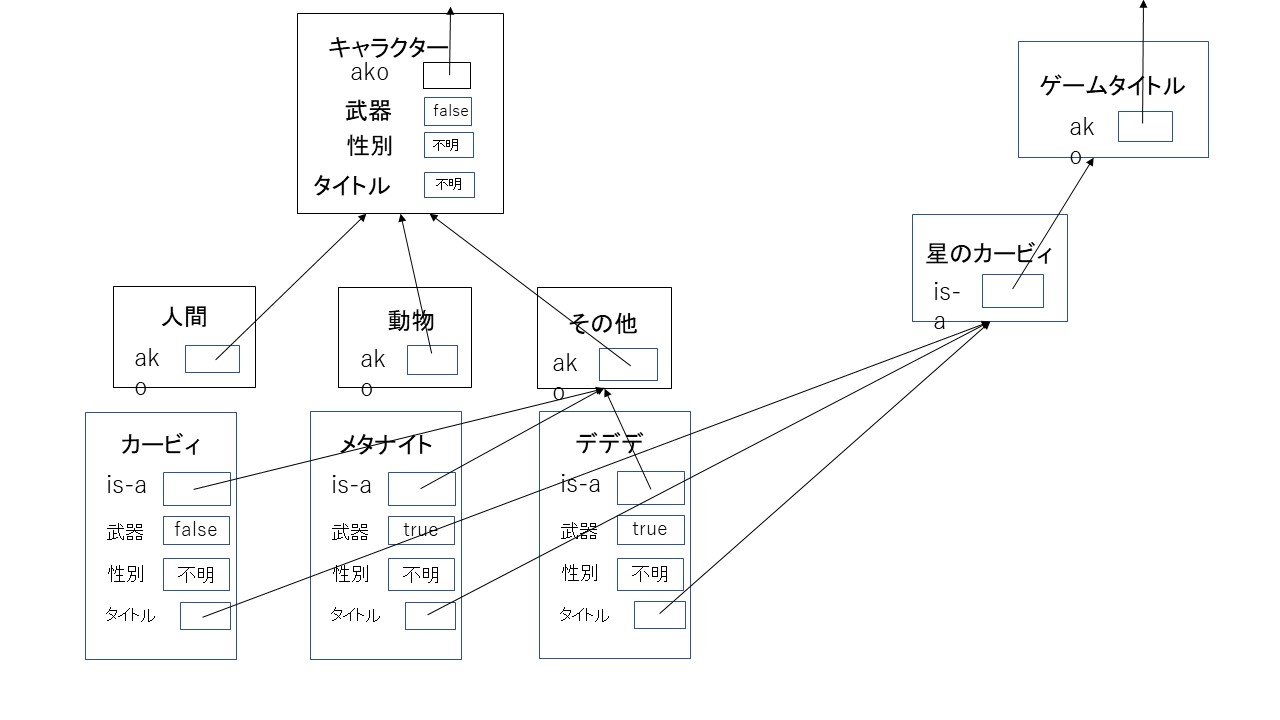
\includegraphics[width=150mm,height=80mm]{095/Frame-Kirby.jpg}

この図において「キャラクター」「人間」「動物」「その他」
「ゲームタイトル」フレームをクラスフレーム、それ以外をインスタンスフレームとして構築している。\\
上に示したフレームを生成する.フレームの生成はExample.javaを元に実装した.\\
実装する上で、ゲームタイトルを加えなければならないため、AIFrameSystem.javaとAIFrame.javaにゲームタイトルを格納するフレームを格納する、取り出すメソッドを加えた。
\subsection{実行例-29114095 野竹浩二朗}
実際にフレームに格納されている値を表示するメソッドを作り、格納されている値を確かめた。次にその1例を示す
\\
\begin{screen}
\begin{verbatim}
Frame:カービィ
武器:false
性別:不明
タイトル:星のカービィ
\end{verbatim}
\end{screen}
他のキャラクターの値も確かめ、示した図と同じフレームを確認することができた。

\subsection{実行例-グループ}
moodleフレームのプログラムのExample.javaを書き換え、FrameExample.javaを作成した。
以下のように共通のスロットを実装し、マリオでテストした。
\begin{lstlisting}
    // クラスフレーム キャラクター の生成
    fs.createClassFrame("キャラクター");
    // 武器 スロットを設定
    fs.writeSlotValue("キャラクター", "武器", Boolean.valueOf(false));
    // クラスフレーム 人間 の生成
    fs.createClassFrame("キャラクター", "人間");
    // クラスフレーム 人間 の生成
    fs.createClassFrame("キャラクター", "動物");
    // クラスフレーム 人間 の生成
    fs.createClassFrame("キャラクター", "その他");
    // クラスフレーム ゲームタイトル の生成
    fs.createClassFrame("ゲームタイトル");
    // クラスフレーム 人間 の生成
    fs.createInstanceFrame("ゲームタイトル", "スーパーマリオ");

    CreateCharactor(fs, "人間", "マリオ", true, true, "スーパーマリオ");
    System.out.println(fs.readSlotValue("マリオ", "武器"));
    System.out.println(fs.readSlotValue("マリオ", "武器",true));
    System.out.println(fs.readSlotValue("マリオ", "タイトル"));
\end{lstlisting}
出力は以下のようになった。
\begin{lstlisting}
    Frame
    true
    false
    スーパーマリオ
\end{lstlisting}
2行目のtrueは武器を所有していることを示し、3行目のfalseはすでに値が代入されていて
書き換えることができなかったことを示し、4行目はマリオが登場するタイトルである。

\section{課題3-3}
\begin{screen}
    課題3-1または3-2で作った知識表現を用いた質問応答システムを作成せよ.
    \\ なお,ユーザの質問は英語や日本語のような自然言語が望ましいが,
    難しければ課題2で扱ったような変数を含むパターン (クエリー) でも構わない. 
\end{screen}
\subsection{手法}
構築したセマンティックネットの中から探索して、答えが得られるようにした。
入力した質問文の中からリンクのタグを抜き出して、それを利用してクエリで解くという形をとった。

\subsection{実装-29114007池口弘尚}
セマンティックネットの作成と自然言語の係り受け解析はグループレポートを参照。
私が担当したのはmainを持つSearchByNLクラスとChunk.getLikeLinkLabels、Link.LabelContains、Sentence.getLikeKeywords、SemanticNet.isLink、Link.HasSameWordを実装した。

Chunk.getLikeLinkLabelsはChunkの中からLinkのラベルになりそうな文字列を取り出すメソッドである。

\begin{lstlisting}[caption=Chunk.getLikeLinkLabels,label=src:getLikeLinkLabels]
public ArrayList<String> getLikeLinkLabels(){
ArrayList<String> list = new ArrayList<String>();
String verb=null;
for (Iterator<Morpheme> iterator = iterator(); iterator.hasNext();) {
    Morpheme morpheme = iterator.next();
    //名詞であり、具体的なものであるとき
    if(morpheme.getPos().equals("名詞")&&morpheme.NETag.equals("O")) {
        //そのまま加える
        list.add(morpheme.surface);
        verb=null;
        continue;
    }
    //動詞のとき
    if(morpheme.getPos().equals("動詞")) {
        list.add(morpheme.base);
        verb=morpheme.surface;
        continue;
    }
    //助動詞のとき
    if(morpheme.getPos().equals("助動詞")) {
        if(verb==null) {
            list.add(morpheme.base);
            verb=morpheme.surface;
            continue;
        }
        verb+=morpheme.surface;
        list.add(verb);
    }
}
return list;
}
\end{lstlisting}

Link.LabelContainsは今までに登録したラベルに含まれているかどうか確かめるメソッドである。
これまでに登録したラベルをLinkの中に静的なメンバー変数として持たせてある。


Sentence.getLikeKeywordsは文の中からLinkのHeadとTailになりそうな文字列を探索するメソッドである。
以下のように実装した。

\begin{lstlisting}[caption=Link.LabelContains,label=LabelContains]
public List<String> getLikeKeywords(Chunk verbChunk){
    List<String> keyList = new ArrayList<String>();
    String preNoun="";
    List<Chunk> chunks = new ArrayList<Chunk>();
    //係り元とそれ自身の文節のみ調べる
    chunks.addAll(verbChunk.getDependents());
    chunks.add(verbChunk);
    for (Chunk chunk : chunks) {
        for (Morpheme morpheme : chunk) {
            //名詞であれば加え、続けて出た場合はつなげたものも加える
            if(morpheme.getPos().equals("名詞")) {
                preNoun+=morpheme.getSurface();
                if(morpheme.getPos(1).equals("接尾"))
                    keyList.add(preNoun);
                else
                    keyList.add(morpheme.getSurface());
            }
            //連体化したものも加える
            else if(morpheme.getPos(1).equals("連体化")) {
                preNoun+=morpheme.getSurface();
            }
            else {
                if(!preNoun.equals("")&&!keyList.contains(preNoun))
                    keyList.add(preNoun);
                preNoun="";
            }
        }
    }
    return keyList;
}
\end{lstlisting}

SemanticNet.isLinkはlabelとkeywordsから変数を持つリンクを作成するメソッドである。
以下のように実装した。

\begin{lstlisting}[caption=SemanticNet.isLink,label=isLink]
public List<Link> isLink(String label, List<String> keywords) {
    List<Link> list = new ArrayList<Link>();
    boolean isHead = false;
    boolean isTail = false;
    for (String key : keywords) {
        for (Link link : links) {
            if (!label.equals(link.getLabel()))
                continue;
            //HeadかTailかは1回ずつのみ
            if (key.equals(link.getHead().getName()) && !isHead) {
                list.add(new Link(label, "?x", key));
                isHead = true;
            } else if (key.equals(link.getTail().getName()) && !isTail) {
                list.add(new Link(label, key, "?x"));
                isTail = true;
            }
        }
        isHead = isTail = false;
    }
    return list;
}
\end{lstlisting}

Link.HasSameWordは同じ要素を持つLinkかどうか確かめるメソッド。
違うlabelで同じ要素を持つことはないのでそれを確かめるためものである。
以下のように実装した。

\begin{lstlisting}[caption=Link.HasSameWord,label=HasSameWord]
public boolean HasSameWord(List<Link> links) {
    String s1 = getHead().toString().startsWith("?")?getHead().toString():getTail().toString();
    for (Link link : links) {
        String s2 = link.getHead().toString().startsWith("?")?link.getHead().toString():link.getTail().toString();
        if(s1.equals(s2))
            return true;
    }
    return false;
}
\end{lstlisting}

探索するためのSearchByNLクラスは以下のように実装した。

\begin{lstlisting}[caption=Link.HasSameWord,label=HasSameWord]
public class SearchByNL {

public static void main(String[] args) {
Scanner stdin = new Scanner(System.in);
String text = "";
SemanticNet sn = MakeSemanticNet.makeSemanticNet();
while (true) {
System.out.println("いらっしゃいませ!いらっしゃいませ!いらっしゃいませ!:");
text = stdin.nextLine();
if (text.equals("exit"))
break;
System.out.println("解析対象のテキスト: " + text);

// 対象テキストを文に分割した上でCaboChaに渡し,解析結果を受け取る.
List<Sentence> sentences = Sentence.parseText(text);
List<List<Link>> linkslist = new ArrayList<List<Link>>();
for (Sentence sentence : sentences) { // 文を1つずつ処理するループ
Sentence.Question q = sentence.getAgentQuestionType();

for (Chunk chunk : sentence) {//文節ごとにループ
for (String likeLabel : chunk.getLikeLinkLabels()) {//ラベルになりそうな文字列を取り出す
if (Link.LabelContains(likeLabel)) {//ラベルかどうか確かめる
List<String> keywords = sentence.getLikeKeywords(chunk);//キーワードを取り出す
List<Link> links = sn.isLink(likeLabel, keywords);//クエリを取り出す
boolean isSame=false;
if(linkslist.size()>0&&likeLabel.equals("だ")&&links.size()>0) {//isを表す"だ"以外を除く
for (Link link : links) {
List<Link> prelinks = linkslist.get(linkslist.size()-1);
if(link.HasSameWord(prelinks)) {
isSame=true;
break;
}
}
}
if (links.size() > 0&&!isSame)
linkslist.add(links);
}
}
}
}
if(linkslist.size()==0)
{
System.out.println("質問がわかりません。");
continue;
}
ArrayList answer = new ArrayList();
answer = checkQuery(sn, answer, linkslist, 0); //答えを検索
if(answer.size()==0)
{
System.out.println("質問がわかりません。");
continue;
}
System.out.print("それは");
for (Object object : answer) {
HashMap<String, String> result = (HashMap) object;
boolean isFirst = true;
for (String s : result.values()) {
if(!isFirst)
System.out.print("と、");
System.out.print(s);
isFirst=false;
}
}
System.out.println("です。");

}
stdin.close();
}

//クエリを組み合わせて答えが出るものを探す
static ArrayList checkQuery(SemanticNet sn, ArrayList<Link> query, List<List<Link>> linkslist, int id) {
if (id == linkslist.size()) {
ArrayList ans = sn.doQuery(query);//答えを出す
if (ans.size() != 0)
return ans;
return query;
}
for (Link link : linkslist.get(id)) {
query.add(link);
ArrayList ans =checkQuery(sn, query, linkslist, id + 1);
if (query != ans)
return ans;
query.remove(query.size()-1);
}
return query;
}

}

\end{lstlisting}

\subsection{実行例}
\begin{lstlisting}
解析対象のテキスト: 酒が好きなのは誰ですか
それは飛世裕貴です。
\end{lstlisting}
この出力は先の課題で示したセマンティックネットの一例に当てはまる。
\subsection{考察-29114007池口弘尚}
ラベルを取り出したり、キーワードを取り出したりする部分は、経験的な手法によって作ったものなので正確性が低いと思われる。
より正確なものにするためには、単語同士の結びつきの強さなどを利用したものなどが考えられる。

また、回答の形式も複数のパターン用意するため、何をきいているのか調べるQuestionクラスなども実装したが、それを利用したプログラムを書く時間がなかった。
これを利用していれば何を変数にすべきかもある程度調べることができると考えられる。

\subsection{手法-29114031大原拓人}
セマンティックネットを構築できる簡単な日本語のみを受け付けて、
それをラベルとリンク元、リンク先に分解して、linkクラスのadd
メソッドに引数として与えられるようにする。

\subsection{実装-29114031大原拓人}
私の担当した部分は、時間内に実行できるコードを作成できなかったので考察のみ示す。
\subsection{考察-29114031大原拓人}
セマンティックネットとして表現し直せる文章はExample.javaの例を用いて
以下の3種類に分けられる。
\begin{description}
    \item[主語+もの+動詞] 「太郎はフェラーリを所有している」
    \item[主語+もの+である] 「太郎は名工大の学生である」
    \item[主語(もの+連体助詞+属性)+もの] 「太郎の趣味は野球である」  
\end{description}
先の2つは文節ごとの名詞のかたまりを抽出してLinkクラスのaddメソッドに
動詞(またはis-a)、主語、ものの順番で引数として渡せばよい。
しかし、3つ目は引数として渡す順番が変わってしまうので
この構文であることを検出しなければならない。また、連体詞「の」を
用いて検出する場合、「名工生の学生は学生である」という文章が
正しく解釈できない。

\section{感想-29114007池口弘尚}
今回は時間がなかったため、あまり深く課題に関わることができなかった。
しかし、自然言語に対する応答の仕方を調べていくと、かなり興味深い内容が多かったので、
課題とは関係なく調べていきたいと思う。
\section{感想-29114031大原拓人}
今回はグループで集まって課題をするための時間を多く作れなかったので、
進捗が遅れてしまった。日本語の構文解析ができるmecabやcabochaを用いたが、
得られる情報が多く混乱してしまった。自分に必要な情報を整理できるようにしたい。
% 参考文献
\begin{thebibliography}{99}
	\bibitem{pl} ウェブインテリジェンスの演習で用いられたコードの例を参考にした
\end{thebibliography}

\end{document}